%% Based on a TeXnicCenter-Template by Tino Weinkauf.
%%%%%%%%%%%%%%%%%%%%%%%%%%%%%%%%%%%%%%%%%%%%%%%%%%%%%%%%%%%%%

%%%%%%%%%%%%%%%%%%%%%%%%%%%%%%%%%%%%%%%%%%%%%%%%%%%%%%%%%%%%%
%% HEADER
%%%%%%%%%%%%%%%%%%%%%%%%%%%%%%%%%%%%%%%%%%%%%%%%%%%%%%%%%%%%%
\documentclass[a4paper,twoside,10pt]{report}
% Alternative Options:
%	Paper Size: a4paper / a5paper / b5paper / letterpaper / legalpaper / executivepaper
% Duplex: oneside / twoside
% Base Font Size: 10pt / 11pt / 12pt


%% Language %%%%%%%%%%%%%%%%%%%%%%%%%%%%%%%%%%%%%%%%%%%%%%%%%
\usepackage[USenglish]{babel} %francais, polish, spanish, ...
\usepackage[T1]{fontenc}
\usepackage[ansinew]{inputenc}
\usepackage{here}

\usepackage{lmodern} %Type1-font for non-english texts and characters


%% Packages for Graphics & Figures %%%%%%%%%%%%%%%%%%%%%%%%%%
\usepackage{graphicx} %%For loading graphic files
\usepackage{subfigure} %%Subfigures inside a figure


\usepackage{amsmath}
\usepackage{amsfonts}


\begin{document}

\pagestyle{empty} %No headings for the first pages.


%% The simple version:
\title{Machine Learning - Homework 2}
\author{Mich�le Wyss}
\date{30.10.2013}
\maketitle

\pagestyle{plain}




\section*{Question 1}
Using few training data, e.g. approx. 3\% out of all available data, GDA works slightly better compared to the linear regression model. The accuracy is in both cases around 50-65\%.
\begin{figure}[ht]
		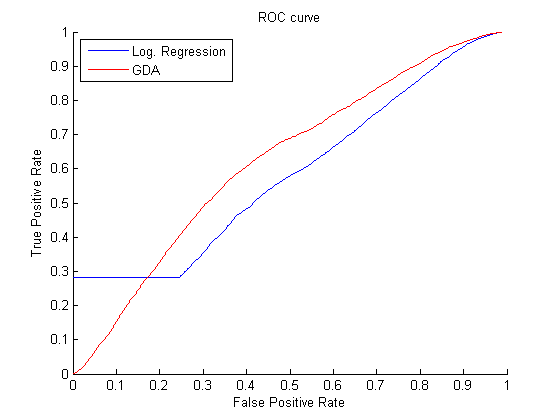
\includegraphics[scale=0.4]{figures/roc-3percent.png}
		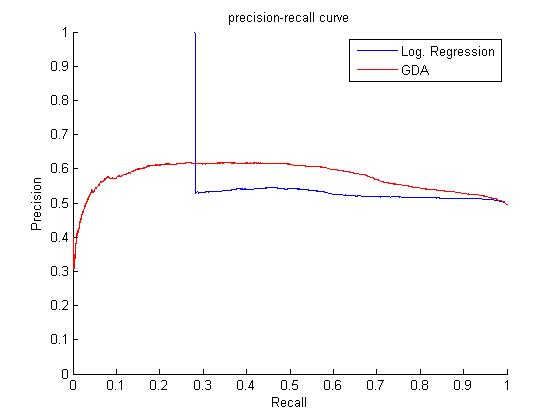
\includegraphics[scale=0.4]{figures/precRec-3percent.png}
\end{figure}

\noindent Since GDA does not yield significantly better results than the Logistic Regression Model I'm not sure whether our data is really gaussian. However, because the results using the GDA are more or less stable (mostly between 52-65\% correct predictions with different but small training sets), I assume that the data is not very far away from the supposed kind of distribution either. \vspace{5mm}

\noindent If we use only slightly more training samples, say 5\% (i.e. about 990 images), the results of both the GDA and the Linear Regression model are not very far from each other and both perform rather badly.
\begin{figure}[ht]
		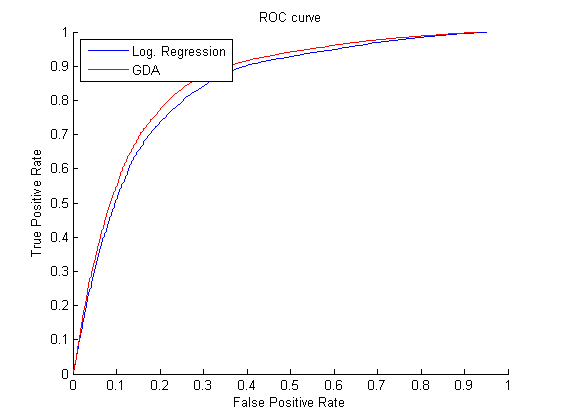
\includegraphics[scale=0.4]{figures/roc-5percent.png}
		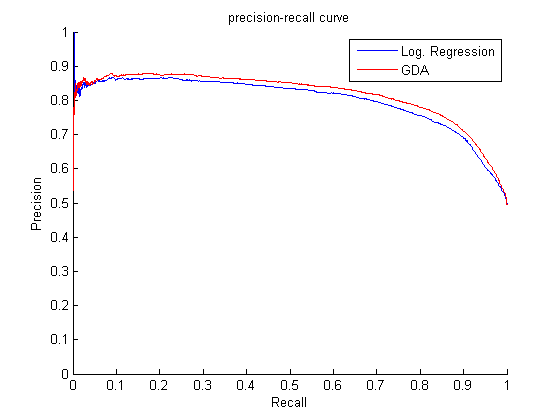
\includegraphics[scale=0.4]{figures/precRec-5percent.png}
\end{figure}

\noindent Trying out the classifiers with many more training samples leads to very similar results for the GDA as for the Linear Regression model.
\begin{figure}[H]
		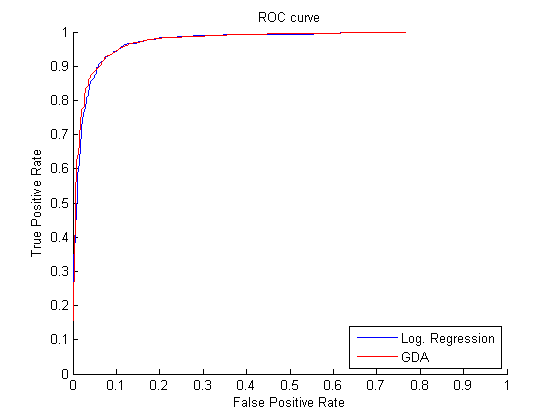
\includegraphics[scale=0.4]{figures/roc-90percent.png}
		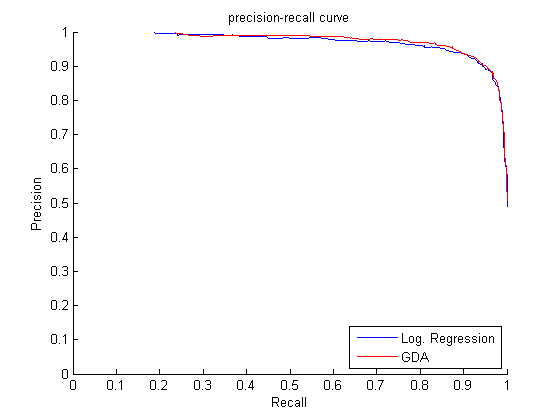
\includegraphics[scale=0.4]{figures/precRec-90percent.png}
\end{figure}
\noindent So on our problem the GDA model works not bad, but I think that it's still not a satisfying accuracy (since the predictions are correct in only ~90\% of the test cases). 

\section*{Question 2}



\end{document}

